%!TEX ROOT = ./main.tex

\section{Experimental Evaluation}\label{sec:experiments}
%\MS{List the specifications of the cluster machine/laptop with which we have run our experiments.}
We evaluate a prototype implementation of ALg.~\ref{alg:abcd-for-tracking}
on two examples. 
The design of nominal controller has been performed on a laptop with core i7-4510u CPU at 3.10GHz, with 8GB of
RAM.
The formal controller synthesis has been performed
on a cluster with 4 Intel Xeon E7-8857 v2 CPUs (48 cores in total) at 3GHz, with 1.5TB of
RAM.
\subsection{Inverted Pendulum}\label{subsec:invpend}
As a simple example, consider the standard problem of designing a controller for a frictionless inverted pendulum.
The goal of the controller is to bring the pendulum to vertical position while satisfying hard constraints on the state variables and control inputs.
A model of the system can be constructed using physical principles. Taking angular position ($\theta$) and angular speed ($\omega$) as state variables, the state vector is represented as $x=\begin{bmatrix}\theta&\omega\end{bmatrix}^\top$ and its dynamics is described as $\dot x(t)\in f^{ip}(x(t),u(t))+W$, where $u(t)$ denotes the input torque, at time $t$ and
\begin{equation}\label{eq:inv_pend_ss}
	f^{ip}(x(t),u(t))=\begin{bmatrix}\omega(t)\\\frac{g}{L}sin(\theta(t))+u(t)\end{bmatrix}.
\end{equation}
%\begin{align*}\label{eq:inv_pend_ss}
%\dot\theta(t)&=r(t)+w_1(t)\nonumber\\
%\dotr(t)&=\frac{g}{L}sin(\theta(t))+u(t)+w_2(t)
%\end{align*}
%bounded with a polyhedral set $w(t)\in W$ for $W\subset\reals^2$, captures the modelling errors. 
The parameter $g=9.81 [m/s^2]$ is the gravitational acceleration
and $L$ is the length of the bar. 

Starting from initial state $x_0^{nom}=\begin{bmatrix}-\pi&0\end{bmatrix}^\top$, the control goal is to converge to an $\varepsilon-$neighbourhood of the equilibrium point 
$x_e=\begin{bmatrix}0&0\end{bmatrix}^\top$. To this end, we first consider the undisturbed system ($W=\{0\}\times \{0\}$)  and use ALTRO to generate a (nominal) trajectory $(x_0^\nom,\ldots,x_K^\nom)$ such that $x_K^{nom}\approx x_e$. Setting the sample time $\tau=0.05[sec]$, $L=9.81[m]$ and $K=100$, generating the nominal trajectory takes 0.14 seconds.



Next, we use SCOTS to implement Alg.~\ref{alg:abcd-for-tracking} in order to synthesize a controller such that nominal trajectory is not violated beyond the specified tube around it under different levels of disturbance. Taking state space $X=[-\pi,\pi]\times[-2,2]$, input space $U=[-0.2,3]$, state space discretization step $\eta_x=\begin{bmatrix}0.001&0.01\end{bmatrix}^\top$ and input space discretization step $\eta_u=0.25$, we use Alg.~\ref{alg:abcd-for-tracking} to compute controllers for various $W$ and $\varepsilon$. Note that the full state space has approx.\ $2.5\times 10^6$ states over which abstraction and controller synthesis take 53.65 seconds and 4.5 seconds, respectively. Table~\ref{tab:inv_pend} demonstrates the effect of changing tube width on size of reduced state space and magnitude of disturbance under which SCOTS is able to find controller. It can be observed that by increasing the tube width, synthesizing a controller for larger disturbance levels is enabled in the cost of increasing size of state space. Fig.~\ref{fig:invpend_traj} demonstrates trajectories of the inverted pendulum system governed by controllers produced by ALTRO and SCOTS when $W=\{0.042\}\times \{0.042\}$ and $\varepsilon=0.06$. As expected, the controller produced by ALTRO is not able to keep the trajectory of the system within the tube around the nominal trajectory, whereas using the controller generated by SCOTS, the trajectory remains within the specified tube.
%Additionally, we require the state constraints $\theta_k\in[-\pi,\pi]$ and $v_k\in[-\pi/8,\pi/8]$ to hold at all time instances.
%\begin{figure}\label{fig:inv_pend}
%	\includegraphics[]{}
%	\caption{Variations of disturbance limit for which SCOTS is able to find a controller with tube size}
%\end{figure}
\begin{figure}[t]\label{fig:invpend_traj}
	\centering
	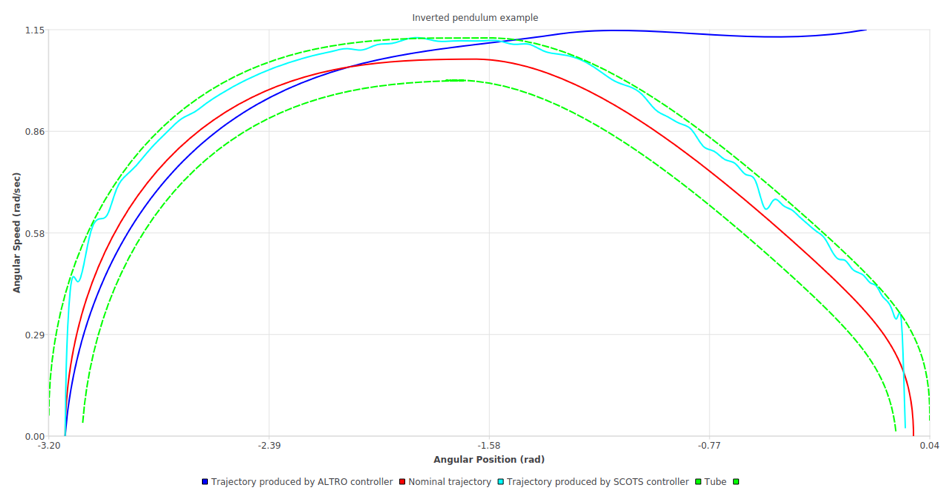
\includegraphics[width=0.85\textwidth]{traj_inv_pend.png}
	\caption{Trajectories of inverted pendulum when open loop controller produced by ALTRO and formally synthesized controller produced by SCOTS were used.}
\end{figure}
\begin{table}[h!]
	\centering
	\caption{Variations in $W$ (disturbance set under which using ALg.~\ref{alg:abcd-for-tracking} a controller can be synthesized), size of state space and required time for abstraction and synthesis for different tube width ($\varepsilon$).}
	\vspace{1mm}
	\begin{tabular}{|c|c|c|c|c|}
		\hline
		$\varepsilon$ &  $W$  & State space size & Abstraction time ([sec])  & Synthesis time ([sec])\\
		\hline
		$\varepsilon<0.02$  & -    & -  & -  &-\\
		\hline
		0.02   & $[-10^{-5},-10^{-5}]^2$    & $14.771\times 10^3$  & 0.24  &0.003\\
		\hline
		0.03   & $[-0.021,0.021]^2$   & $27.206 \times 10^3$ & 0.41  &0.013\\
		\hline
		0.04    & $[-0.048,0.048]^2$  & $39.952\times 10^3$  & 0.73  &0.038\\
		\hline
		0.05  &  $[-0.055,0.055]^2$   & $52.648 \times 10^3$  & 0.92 &0.058 \\
		\hline
		0.06    & $[-0.061,0.061]^2$  & $65.347 \times 10^3$  & 1.21  &0.077\\
		\hline
		0.07   &$[-0.067,0.067]^2$  & $78.183 \times 10^3$     & 1.51 &0.099\\
		\hline
		0.08   &$[-0.068,0.068]^2$  & $90.490 \times 10^3$     & 1.82 &0.13\\
		\hline
	\end{tabular}
	\label{tab:inv_pend}
\end{table}
\subsection{Ship Docking}\label{subsec:6dship}
Next, we consider controller synthesis for a ship docking scenario wherein a ship starts moving toward the dock from a certain distance and the control goal is hence to bring the ship from its start point into the dock such that the ship's speed near the dock is very small. To represent the ship's model in state space, we partition the state vector as $x=\begin{bmatrix}\lambda& \nu\end{bmatrix}^\top$, where $\lambda=\begin{bmatrix}N&E&\psi\end{bmatrix}^\top$ are the South-North and West-East positions and heading of the ship, $\nu = \begin{bmatrix}g &h&k\end{bmatrix}^\top$ are the surge and sway velocities, and yaw rate of the ship. Moreover, we consider disturbance due to current velocities ($W_c\subset\reals^3$) and disturbance corresponding to wind forces ($W_{wind}\subset\reals^3$ ). One can write the ship dynamics as $\dot x(t)\in f^s(x(t),u(t))+W$, where $u\in\reals^3$ and $W=W_c\times W_{wind}$ denote the control input vector and disturbance set and
\begin{equation}\label{eq:ship_ss}
f^{s}(x(t),u(t))=\begin{bmatrix}R(\psi)\nu\\M^{-1}(u(t)-C(\nu)\nu-D\nu)\end{bmatrix}.
\end{equation}
%The state space equations of the ship model are
%\begin{align*}
%&\dot{\eta}=R(\psi)\nu+w_c \\
%&M\dot{\nu}+C(\nu)\nu+D\nu=u+R(\psi)^{\top}w_{wind},
%\end{align*}
where $R=R(\psi)=\begin{bmatrix}
cos(\psi) &-sin(\psi) &0\\
sin(\psi) & cos(\psi) & 0\\
0 & 0 & 1
\end{bmatrix}$ is a rotation matrix. Further, the inertia matrix $M=\begin{bmatrix}
87.4 & 0 & 0 \\
0 & 98.3 & 2.48 \\
0 & 2.48 & 22.2
\end{bmatrix}$, the damping matrix $D=\begin{bmatrix}
6.58 & 0 & 0 \\
0 & 37.7 & 2.66 \\
0 & 2.66 & 19.3
\end{bmatrix}$ and Coriolis matrix $C(v)=\nu(1)\begin{bmatrix}
0 & 0 & 0 \\
0 & 0 & 98.3 \\
0 & 0 & 2.48
\end{bmatrix}$ are chosen for a $1:30$ scale model of a platform supply vessel.

Starting from an initial state $x_0^{nom}=\begin{bmatrix}0&0&0&0&0&0\end{bmatrix}^\top$, the control goal is to converge to $\varepsilon-$neighbourhood of the point 
$x_d=\begin{bmatrix}1&1&0&0&0&0\end{bmatrix}^\top$. We first consider the undisturbed system and use ALTRO to generate a (nominal) trajectory $(x_0^\nom,\ldots,x_K^\nom)$ such that $x_K^{nom}\approx x_d$. Setting the time step $\tau=3[sec]$, and $K=8$, generating the nominal trajectory takes around 3.16 seconds. Next, we use SCOTS in order to synthesize a controller such that the nominal trajectory is not violated beyond $\varepsilon$, under different levels of disturbance. Taking state space $X=[-.3,1.25]^2\times[-.3,.7]\times[-.03,.12]\times[-.03,.075]\times[-.085,.095]$, input space $U=[-2,2]^3$, state space discretization step $\eta_x=\begin{bmatrix}.05&.05&.05&.005&.005&.005\end{bmatrix}^\top$ and input space discretization step $\eta_u=\begin{bmatrix}.5&.5&.5\end{bmatrix}^\top$, we used ALg.~\ref{alg:abcd-for-tracking} to compute controller for $\varepsilon=2\eta_s$ and $W=[-.001,.001]^3\times[-.0001,.0001]^3$. By decreasing size of state space from $5.4\times 10^8$ into $4.5*10^6$, abstraction and synthesis over reduced state space take $1539.28$ and $413.726$ seconds, respectively. Surprisingly, abstraction and synthesis for full state space could not be performed on our cluster machine in this example.

%\textcolor{red}{
\subsection{Multi Agent Problem}\label{sec:MultiAgent}
In this example, we are solving a controller design problem for a multi agent systems. The multi agent system consist of 10 unicycle model . Each agent should start from own initial point and reach target set (which is shown in Fig. \ref{fig:MA}) while it avoids obstacles and collision with other agents. each unicycle has radius $0.1$. Unicycle model is described in below.
\begin{equation}\label{eq:unicycle_ss}
	f^{u}(x(t),u(t))=
	\begin{bmatrix}
	u_1cos(x_3)\\
	u_1sin(x_3)\\
	u_2
	\end{bmatrix}.
\end{equation}
In Eq. \ref{eq:unicycle_ss} $u_1$ is linear speed and $u_2$ is  angular speed and $x_1$ and $x_2$ represents positions and $x_3$ is the angle. Here goal of the problem is designing a controller which can do the reach avoid task for all of 10 unicycles at same time without having collision with each other. For this purpose, at first we combine all of unicycle dynamics to create a centralized model of the multi agent system. The centralized model has $10\times3$ dimension for state space and $10\times2$ dimension for input space. For initial state of centralized dynamic we combine all of initial states in order(For goal state we do it as well). Collision in the centralized model is modelled with avoiding with the Obstacles configuration below:\\
\begin{equation}
\forall i,j \in [1,10]: \sqrt{(x_i-x_j)^2+(y_i-y_j)^2}< \gamma
\end{equation}
In next step we solve the problem for the setup without disturbance to design an open loop controller for the centralized multi agent system (generating a nominal trajectory). ALTRO solved the problem in 138 seconds with $\gamma=1.5$ and $\tau=0.05$ and 200 knots trajectory points. Result of ALTRO is illustrated in fig \ref{fig:MA}. 
In next step we obtain close loop controller using SCOTS. As we mentioned in Prob. \ref{alg:abcd-with-time-for-tracking} we are able to design a controller that is able to track the trajectory with $\varepsilon$ distance in every time step. Therefore we are able to split the centralized system to 10 separate system and design a close loop controller for each one of them separately. In order to do this step, we select $\varepsilon$ in a way that it satisfies $\gamma> 2\varepsilon$ (since tubes should not intersect with each other). Then we are able to design a formally guarantied controller for each agent independently with Alg. \ref{alg:abcd-with-time-for-tracking} and SCOTS. We select parameters in this way:\\
$\varepsilon=0.32$\\
$\widetilde{X}=[-1:11]*[-1:11]*[-\pi,\pi]*[0,1]$\\
$U=[-3,3]*[-3,3]$\\
$\eta_{\widetilde{X}}=[0.04,0.04,0.04,0.05]$\\
$\eta_{U}=[0.6,0.6]$\\
Controller designed in this way is able to overcome bounded additive disturbance $w=[0.03,0.03,0.03]$. Nominal controller with presence of this disturbance will be pushed outside of the tube. As it shown in the Fig.\ref{fig:MA}, trajectory 1 and 2 will have collision with this value of disturbance(using nominal controller) . Abstraction in total for 10 systems takes about 12 minutes(average 100 seconds for each system) and synthesizing controller takes about 2 minutes(near 10 seconds for each system).
\begin{figure}[t]\label{fig:MA}
	\centering
	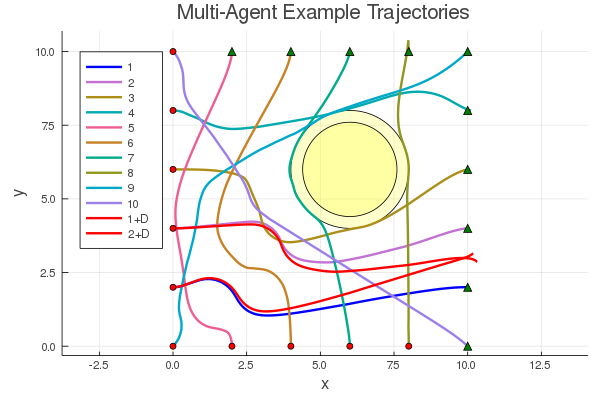
\includegraphics[width=0.85\textwidth]{MA.png}
	\caption{Trajectories of multi agent unicycle when open loop controller produced by ALTRO and formally synthesized controller produced by SCOTS were used.}
\end{figure}




 %Figure~\ref{fig:inv_pend} demonstrates variations of disturbance limit under which SCOTS is able to find a controller for different tube width. %It can be observed that by increasing the tube width, SCOTS is able to synthesize a controller for larger disturbance levels. Figure~\ref{fig:invpend_traj} demonstartes trajectories of the system  \eqref{eq:inv_pend_ssq} governed by controllers synthesized by ALTRO and SCOTS under appliance of constant disturbance vector \MS{$[??,??]$}. As expected, the controller designed by ALTRO is not able to tackle disturbance, while using the controller generated by SCOTS, the trajectory remains within the desired bound.

%\begin{figure}\label{fig:inv_pend}
%	\includegraphics[]{}
%	\caption{Variations of disturbance limit for which SCOTS is able to find a controller with tube size}
%\end{figure}
%\begin{figure}\label{fig:invpend_traj}
%	\includegraphics[]{}
%	\caption{}
%\end{figure}
%\textcolor{red}{
\subsection{Cart-pole and 1D vehicle}
In this example, we show the method can handle multiple heterogeneous dynamical systems. Here we design controller for 2 systems: 1- a cart pole system with dynamics given in \cite{6313077} 2- a vehicle with dynamics 
$\begin{bmatrix} \dot{x_1}\\ \dot{x_2} \end{bmatrix}=\begin{bmatrix} x_2\\ u \end{bmatrix}  $.
$x_1$ represent position and $x_2$ speed. The process of controller synthesize is similar to Sec. \ref{sec:MultiAgent}; At first we make the centralized dynamics by combining dynamics. In the next step we define constraints(obstacles) and solve trajectory generation problem without presence of disturbance. In the final step, we use our method using SCOTS to synthesize robust controller which can track the trajectory with a bounded error.  
%} 



\section{Present Challenges}

\begin{enumerate}
	\item In some examples, it was necessary to consider a larger control input space for the SCOTS part, than what was used in the ALTRO part.
	Otherwise, the SCOTS would not be able to track the nominal trajectory within the given precision using any level of discretization. 
	\item For the ship example, applying the largest disturbance with which SCOTS is able to compute a controller, the trajectory resulted from using the open loop controller does not leave  $\varepsilon-$tube around it; in general magnitude of disturbance for which SCOTS can find a controller is relatively small for most of examples that we have tried.
\end{enumerate}



